\chapter{Polarização da luz}
\textsl{{\sffamily(Versão: \today)}}

\noindent
O termo ``polarização'' refere-se à direção da função de onda, quando a onda é
descrita por funções vetoriais. No caso das ondas eletromagnéticas, a
direção do campo elétrico que usamos para descrever a onda (mas o mesmo se passa
com o campo magnético) é perpendicular à direção de propagação, e por isso
dizemos que as ondas eletromagnéticas são transversais. Dentro do plano
perpendicular à direção de propagação em que está confinada, a orientação da
polarização de uma onda eletromagnética pode ainda variar continuamente e pode
até variar com o tempo e com a posição ao longo do caminho da onda.  Chama-se
\emph{plano de polarização} de uma onda eletromagnética ao plano definido pelas
direções de polarização e de propagação (veja a Figura~\ref{fig:polpln}).
\begin{figure}[htb]
    \small
    \sffamily
    {\centering
    \def\zangle{-20}
    \def\xangle{20}

    \begin{tikzpicture}[x=(\xangle:0.75cm), y=(90:1cm), z=(\zangle:1.5cm),
                        >=stealth, line cap=round
                       ]

        \pgfmathsetmacro{\npts}{192}
        \pgfmathsetmacro{\nwvs}{3}
        \pgfmathsetmacro{\dang}{360*\nwvs/\npts}
        \pgfmathsetmacro{\phi}{60}
        \pgfmathsetmacro{\cosphi}{cos \phi}
        \pgfmathsetmacro{\sinphi}{sin \phi}

        \draw [very thin](0,-1,0) -- (0,1,0);
        \draw [very thin](-1,0,0) -- (1,0,0);
        \draw [->] (0,0,0) -- (0,0,\nwvs+0.25) node[below right] {$\vec k$};

        \draw [dashed,fill=gray!25,ultra thin, fill opacity=0.5]
                (\cosphi,\sinphi,0) -- (-\cosphi,-\sinphi,0) --
                (-\cosphi,-\sinphi,\nwvs+.1) -- (\cosphi,\sinphi,\nwvs+.1) --
                cycle;

        \foreach \k [evaluate={%
              \d=int(\k+1/4);
              \i=\k*\dang;
              \j={\i>0 ? \i+\dang : 0};
              \a=\i; 
              \b=\j; 
              \c=int(mod(\k,8)==0 && cos \a != 0); 
              }]
            in {0,...,192}{

            \draw [semithick](\cosphi*cos \a, \sinphi*cos \a, \i/360) -- 
              (\cosphi*cos \b, \sinphi*cos \b, \j/360);

            \ifnum\c=1
                \draw [->] (0,0,\i/360) --
                    ++(\cosphi*cos \a, \sinphi*cos \a, 0);
            \fi
        }
        \node at (\cosphi,\sinphi,0)   [anchor=south] {$\vec E$};
        \node at (\cosphi,\sinphi,0.5) [anchor=south west,yslant=tan(\zangle)] 
          {\footnotesize Plano de polariza\c{c}\~ao};
    \end{tikzpicture}\par
}
\caption{Plano de polarização de uma onda eletromagnética. O campo magnético não
está representado.\label{fig:polpln}}
\end{figure}
Quando a orientação do plano de polarização de uma onda eletromagnética se
mantém constante, dizemos que a onda está polarizada linearmente. Mas também
pode acontecer que o plano de polarização sofra uma rotação em torno da direção
de propagação, completando uma volta completa ao longo de um comprimento de
onda. Nesse caso dizemos que a onda tem polarização elítica. Vamos já de seguida
estudar estas duas situações.

\section{Polarização linear e polarização elítica}
Numa onda plana com polarização linear, a orientação do plano de polarização
é constante, ou seja, a direção de polarização (que é, recordemos mais uma vez,
a do campo elétrico) deve ser a mesma em todos os pontos do trajeto da onda e em
todos os instantes.

Consideremos uma onda plana sinusoidal com vetor de onda $\vec k$ e
frequência $\omega$. Para simplificar a linguagem, escolhemos a origem dos
tempos de tal modo que a constante de fase é nula e adotamos um referencial com
o eixo dos $z$ orientado segundo o vetor de onda. O plano $xy$ é então
perpendicular à direção de propagação. Seja $E_0$ o módulo da amplitude do campo
elétrico desta onda e $\theta$ o ângulo que a direção de polarização faz com o
eixo dos $x$. Então, o vetor amplitude desta onda é $\vec
E_0=E_0(\cos\theta,\,\sin\theta,\,0)= E_0(\cos\theta\,\he_x+\sin\theta\,\he_y)$,
e a função de onda assume a forma
\begin{equation*}
\vec E(\vec r,t)=E_0(\cos\theta\,\he_x+\sin\theta\,\he_y)
\cos(\vec k\cdot\vec r-\omega t).
\end{equation*}
Podemos ver esta onda como a sobreposição de duas ondas polarizadas linearmente
segundo as direções coordenadas $x$ e $y$ (ver a Figura~\ref{fig:pollin}):
\begin{equation}\label{eq:lpdec}
\vec E(\vec r,t)=\vec E_x(\vec r,t)+\vec E_y(\vec r,t),\qquad\text{com }
\begin{cases}
\vec E_x(\vec r,t)=E_0\cos\theta\,\he_x\,\cos(\vec k\cdot r-\omega t)\\
\vec E_y(\vec r,t)=E_0\sin\theta\,\he_y\,\cos(\vec k\cdot r-\omega t)
\end{cases}
\end{equation}
\begin{figure}[htb]
{\centering
  \def\zangle{210}
  \def\xangle{-10}
  \begin{tikzpicture}[x=(\xangle:1cm), y=(90:1cm), z=(\zangle:1.5cm),
                      >=stealth, line cap=round
                     ]

    \pgfmathsetmacro{\npts}{192}
    \pgfmathsetmacro{\nwvs}{2}
    \pgfmathsetmacro{\dang}{360*\nwvs/\npts}
    \pgfmathsetmacro{\phi}{120}
    \pgfmathsetmacro{\cosphi}{cos \phi}
    \pgfmathsetmacro{\sinphi}{sin \phi}

    \draw [very thin,->](0,-1,0) -- (0,1,0) node [right]{$y$};
    \draw [very thin,->](-1,0,0) -- (1,0,0) node [below]{$x$};
    \draw [->] (0,0,0) -- (0,0,\nwvs+0.25) node[below right] {$z$};
    \fill [fill=gray!25, fill opacity=0.5]
        (-1.1,-1,\nwvs+1) -- (1.1,-1.1,\nwvs+1) --
        (1.1,1.1,\nwvs+1) -- (-1.1,1,\nwvs+1) -- cycle;
    \draw [ultra thin] (-1,0,\nwvs+1)--(1,0,\nwvs+1);
    \draw [ultra thin] (0,-0.97,\nwvs+1)--(0,0.97,\nwvs+1);
    \draw [<->] (-\cosphi,-\sinphi,\nwvs+1) coordinate(e1)--(\cosphi,\sinphi,\nwvs+1)coordinate(e2) node[left]{$\vec E$};
    \draw [<->] (-\cosphi,0,\nwvs+1) coordinate(x1) -- (\cosphi,0,\nwvs+1) coordinate(x2);
    \draw [ultra thin, dashed] (e1)--(x1);
    \draw [ultra thin, dashed] (e2)--(x2) node[yshift=-4mm]{$\vec E_x$};
    \draw [<->] (0,-\sinphi,\nwvs+1)coordinate(y1) -- (0,\sinphi,\nwvs+1)coordinate(y2);
    \draw [ultra thin, dashed] (e1)--(y1);
    \draw [ultra thin, dashed] (e2)--(y2) node[below right]{$\vec E_y$};

    \draw [ultra thin] (0.3,0,\nwvs+1) arc(0:\phi:0.3);
    \path (0.5,0,\nwvs+1) arc(0:\phi/2:0.5) node{$\theta$};
    \draw [ultra thin] (0.3,0,0) arc(0:\phi:0.3);
    \path (0.5,0,0) arc(0:\phi/2:0.5) node{$\theta$};

    \foreach \k [evaluate={%
          \d=int(\k+1/4);
          \i=\k*\dang;
          \j={\i>0 ? \i+\dang : 0};
          \a=\i; 
          \b=\j; 
          \c=int(mod(\k,4)==0 && cos \a != 0); 
          }]
        in {0,...,192}{

        \draw [semithick](\cosphi*cos \a, \sinphi*cos \a, \i/360) -- 
          (\cosphi*cos \b, \sinphi*cos \b, \j/360);

        \ifnum\c=1
            \draw [ultra thin](0,0,\i/360) --
                ++(\cosphi*cos \a, \sinphi*cos \a, 0);
        \fi
    }

  \end{tikzpicture}\par
}
\caption{Decomposição ortogonal da polarização linear de uma onda. Podemos ver
uma onda com polarização linar arbitrária como a soma de duas ondas com
polarizações lineares segundo as direções coordenadas com diferença de fase
nula.\label{fig:pollin}}
\end{figure}

A eq.~\eqref{eq:lpdec} apresenta uma onda eletromagnética com polarização linear
como a sobreposição de duas ondas com a mesma frequência e a mesma fase,
polarizadas linearmente em duas direções ortogonais. Trata-se de um exemplo
particular (para o caso de iguais frequências e fases) da sobreposição de
movimentos oscilatórios ortogonais, cuja resultante é, em geral, conhecido como
\emph{figura de Lissajous.}

As duas componentes da decomposição da polarização linear descrita na
eq.~\eqref{eq:lpdec} têm diferença de fases nula, e resulta da sobreposição uma
onda polarizada linearmente. Mas consideremos agora o que acontece quando as
duas componentes ortogonais da polarização têm uma diferença de fase
$\delta\varphi\neq0$. A diferença de fase entre as duas componentes geram uma
sobreposição com orientação que roda em torno da direção de propagação,
completando num dado ponto uma volta completa durante um período ou, num dado
instante, realizando uma rotação ao longo de um comprimento de onda. Porque o
plano de polarização vai rodando ao longo da direção de propagação, a
extremidade do vetor amplitude desenha, no plano perpendicular a essa direção
uma figura fechada com a forma de uma elipse. Por esta razão, dizemos que ondas
com este comportamento têm \emph{polarização elíptica.} A excentricidade desta
elipse depende das amplitudes das duas componentes do campo e também da
diferença entre as as fases das duas ondas. A Figura~\ref{fig:circpol} tenta
ilustrar esta rotação da direção de polarização nas ondas com polarização
elíptica. Note-se que a figura representa apenas a \emph{amplitude} do campo
elétrico, não a parte que depende mais explicitamente do tempo e da posição. 
\begin{figure}[htb]
{\centering
\def\zangle{220}
\def\xangle{-10}
\begin{tikzpicture}[x=(\xangle:1cm), y=(90:1cm), z=(\zangle:1.25cm),
                      				>=stealth, line cap=round
                     			   ]
\small
\pgfmathsetmacro{\n}{200}
\pgfmathsetmacro{\tm}{850}
\pgfmathsetmacro{\dt}{\tm/\n}
\pgfmathsetmacro{\zm}{4}
\pgfmathsetmacro{\dz}{\zm/\n}

\draw [very thin,->](0,-1,0) -- (0,1,0) node [right]{$y$};
\draw [very thin,->](-1,0,0) -- (1,0,0) node [below]{$x$};
\draw [thick,->] (0,0,0) -- (0,0,1.1*\zm) node[below right] {$z$};

\foreach \k 
[evaluate={
						\t = \k*\dt;
						\tp = \dt*(\k+1);
						\z=\k*\dz;
						\flag=int(mod(\k,4)==0);
						}]
 in {0,...,\n}{
		\draw [semithick]({cos(\t)},{sin(\t)},\z)--({cos(\tp)},{sin(\tp)},{\z+\dz});
		\ifnum\flag=1
			\draw [ultra thin] (0,0,\z) -- ({cos(\t)},{sin(\t)},\z);
		\fi
	}
    \fill [fill=gray!25, fill opacity=0.5]
        (-1.1,-1,\zm+1.5) -- (1.1,-1.1,\zm+1.5) --
        (1.1,1.1,\zm+1.5) -- (-1.1,1,\zm+1.5) -- cycle;
		\draw (0,0,\zm+1.5) circle (1);
		\draw [->] (0,0,\zm+1.5) -- ({cos(\tm)},{sin(\tm)},\zm+1.5)
        node[yshift=-4mm]{$\vec E_0$};
		\draw [->] ({1.1*cos(\tm-10)},{1.1*sin(\tm-10},\zm+1.5) 
        arc(\tm-10:\tm+10:1.1);
\end{tikzpicture}\par
}
\caption{Rotação do plano de polarização numa onda com polarização elítica.
Para manter a figura o mais clara possível, apenas está representada a amplitude
do campo elétrico e não o campo elétrico propiamente dito, que inclui ainda o
usual fator ondulatório $\cos(\vec k\cdot r-\omega t)$.\label{fig:circpol}}
\end{figure}

Em geral, a sobreposição das duas componentes ortogonais do campo elétrico é
semelhante à construção matemática que produz as chamadas figuras de Lissajous,
com frequências iguais. Veja a Secção~\ref{sec:lissajous} para uma revisão rápida das figuras
de Lissajous.

\section{Filtros polarizadores e Lei de Malus}
\tobedone{}
\section{Polarização por reflexão e por difusão}
\tobedone{}
\section{Birefrigência}
\tobedone{}
\section{Aplicações na optometria}
\tobedone{}

\section{Apêndice: figuras de Lissajous com frequência única}
\label{sec:lissajous}
Consideremos o movimento de um ponto material no plano $xy$ cujas coordenadas
são dadas por 
\begin{align}\label{eq:mcu}
x(t)&=r\cos\omega t&y(t)=r\sin\omega t,
\end{align}
com $r$ e $\omega$ constantes positivas. É claro que este ponto descreve um
movimento circular uniforme, com raio $r$ e velocidade angular $\omega$ (veja a
Figura~\ref{fig:mcu}).
\begin{figure}[htb]
{\centering
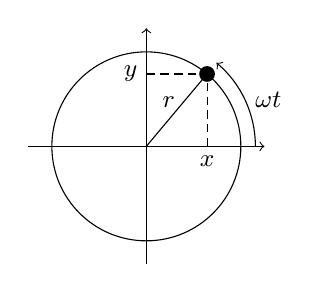
\begin{tikzpicture}
  \small
  \coordinate (O) at (0,0);
  \draw [->] (-1.5,0) -- (1.5,0);
  \draw [->] (0,-1.5) -- (0,1.5);
  \def\r{1.2}
  \def\theta{50}
  \draw [thin] (O) circle (\r);
  \fill (\theta:\r) coordinate(P) circle(0.1);
  \draw [thin,->] (0:\r+.185) arc (0:\theta:\r+.185);
  \node at (0.5*\theta:\r+0.2) [anchor=west] {$\omega t$};
  \draw [thin, densely dashed] (O-|P)node[below]{$x$} -- (P) --
        (P-|O) node [left]{$y$};
  \draw [thin] (O) -- (P) node [midway, shift={(-.1,.1)}] {$r$};
\end{tikzpicture}\par
}
\caption{Movimento circular e uniforme de um ponto com coordenadas que dependem
do tempo de acordo com as eqs.~\eqref{eq:mcu}.\label{fig:mcu}}
\end{figure}
Tendo em conta que $\sin\theta=\cos(\theta-\pi/2)$, as expressões das
coordenadas do ponto em estudo, das eqs.~\eqref{eq:mcu}, podem também
escrever-se como
\begin{align}
x(t)&=r\cos\omega t& y(t)&=r\cos(\omega t-\pi/2).
\end{align}

Façamos agora uma generalização destas expressões, substituindo o valor $\pi/2$
na segunda igualdade por um parâmetro genérico $\varphi,$ e analisemos as
trajetórias da família definida pelas igualdades
\begin{align}\label{eq:mcu2}
x(t)&=r\cos\omega t& y(t)&=r\cos(\omega t-\varphi).
\end{align}
O caso $\varphi=\pi/2$ é o que já vimos. A trajetória correspondente é uma
circunferência descrita no sentido anti horário. Mas há outras possibilidades.
Por exemplo, com $\varphi=0$ tem-se $x(t)=y(t);$ a trajetória resultante é então
um segmento de reta com inclinação 45$^\circ$, percorrido pelo ponto material
alternadamente num sentido e no sentido inverso.  Com $\varphi=\pi$, a situação
é muito semelhante (mas agora $y(t)=-x(t)$); resulta uma trajetória também
retilínea, mas com inclinação $-45^\circ$. Para $\varphi=-\pi/2$ resulta
novamente uma trajetória circular, mas descrita em sentido horário. Mais em
geral, a trajetória resultante é uma elipse mais ou menos excêntrica, com uma
inclinação $\pm45^\circ$\footnote{O applet geogebra \texttt{lissajous} em
\texttt{https://ggbm.at/zbC56YsK} ajuda na exploração
das várias possibilidades.}.  A Figura~\ref{fig:lsjx_examples} ilustra os casos
agora referidos e ainda o caso $\varphi=\pi/4$.
\begin{figure}[htb]
{\centering
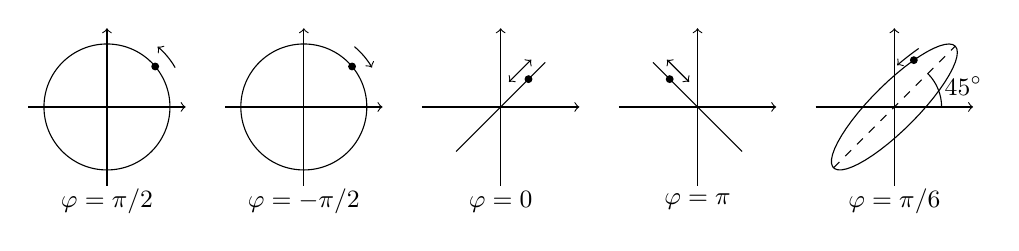
\begin{tikzpicture}
    \small
	\def\r{0.8}
	\def\q{40}
	\begin{scope}[xshift=-5cm]
		\draw [->,thin] (-1,0) -- (1,0);
		\draw [->,thin] (0,-1) -- (0,1);
		\draw [thin] (0,0) circle(0.8);
		\fill(\q:\r) circle(0.05);
		\draw [->] (\q-10:\r+0.2) arc(\q-10:\q+10:\r+.2);
		\node at (0,-1.2) {$\varphi=\pi/2$};
	\end{scope}
	\begin{scope}[xshift=-2.5cm]
		\draw [->,thin] (-1,0) -- (1,0);
		\draw [->,thin] (0,-1) -- (0,1);
		\draw [thin] (0,0) circle(0.8);
		\fill(\q:\r) circle(0.05);
		\draw [->] (\q+10:\r+0.2) arc(\q+10:\q-10:\r+.2);
		\node at (0,-1.2) {$\varphi=-\pi/2$};
	\end{scope}
	\begin{scope}[xshift=0cm]
		\draw [->,thin] (-1,0) -- (1,0);
		\draw [->,thin] (0,-1) -- (0,1);
		\draw (225:\r) -- (45:\r);
		\fill (45:0.5)coordinate(p) circle(0.05);
		\path (p)--++(225:0.2)--++(135:0.15) coordinate(q);
		\draw [<->] (q) --++(45:0.4);
		\node at (0,-1.2) {$\varphi=0$};
	\end{scope}
	\begin{scope}[xshift=2.5cm]
		\draw [->,thin] (-1,0) -- (1,0);
		\draw [->,thin] (0,-1) -- (0,1);
		\draw (135:\r) -- (315:\r);
		\fill (135:0.5)coordinate(p) circle(0.05);
		\path (p)--++(315:0.2)--++(45:0.15) coordinate(q);
		\draw [<->] (q) --++(135:0.4);
		\node at (0,-1.2) {$\varphi=\pi$};
	\end{scope}
	\begin{scope}[xshift=5cm]
		\draw [->,thin] (-1,0) -- (1,0);
		\draw [->,thin] (0,-1) -- (0,1);
    \draw [domain=0:360,samples=50,variable=\t] 
      plot ({\r*cos(\t)},{\r*cos(\t-30)});
    \fill ({\r*cos(72)},{\r*cos(42)}) circle(0.05);

    \draw [->,domain=72:88,samples=5,variable=\t] 
        plot ({(\r+.2)*cos(\t)},{(\r+.2)*cos(\t-30)});
		\node at (0,-1.2) {$\varphi=\pi/6$};
    \draw [thin,dashed]
    ({\r*cos(195)},{\r*cos(165)})--({\r*cos(15)},{\r*cos(-15)});
    \draw (0:0.6) arc(0:45:0.6) node [shift=({1mm,0.75mm}),anchor=north west]
            {$45^\circ$};
	\end{scope}
\end{tikzpicture}\par
}
\caption{Alguns exemplos de sobreposição ortogonal de dois movimentos
oscilatórios com a mesma frequência e amplitude.\label{fig:lsjx_examples}}
\end{figure}

As figuras planas resultantes de sobreposição de movimentos oscilatórios em
direções perpendiculares chama-se \emph{Figuras de Lissajous.} Nestes
apontamentos consideramos apenas o caso em que as frequências de ambos os
movimentos são iguais, por ser o relevante para o estudo da polarização elítica.

Estudámos aqui a situação mais simples, em que as amplitudes dos dois movimentos
oscilatórios são iguais. Mas, no essencial, as coisas não se alteram grandemente
quando as amplitudes são diferentes, excepto no seguinte:
\begin{enumerate}
\item
  Se as amplitudes dos dois movimentos são diferrentes, a trajetória resultante
  nunca chega a ser exatamente circular, permanece sempre elítica acom maior ou
  menor excentricidade;
\item
  Se as amplitudes dos dois movimentos são diferentes, a inclinação do eixo da
  elipse pode tomar outros valores para além de $\pm45^\circ$, obtidos acima.
\end{enumerate}
